%%%%%%%%%%%%%%%%%%%%%%%%%%%%% TCC %%%%%%%%%%%%%%%%%%%%%%%%%%%%%%%%
%
% Template para TCC da Universidade Federal da Paraíba
%
% Autores: Elaine Soares elaineanita1@gmail.com
%          Rafael Brayner rafabrayner92@gmail.com
%          Roberto Júnior contato@robertojunior.net
%
% ShareLaTeX porting: Gustavo Sobral ghsobral@gmail.com
% 
% Revisão: Eudisley Anjos eudisley@ci.ufpb.br
%
% Sinta-se livre para melhorar e contribuir com esse projeto. 
%
%%%%%%%%%%%%%%%%%%%%%%%%%%%%%%%%%%%%%%%%%%%%%%%%%%%%%%%%%%%%%%%%%%%

\documentclass{tcc}

\begin{document}
\pagestyle{empty} %retira numeração da página
%Dados do TCC%
\author{Willian Marques Freire}
\title{IoT e integração com Micro-serviços}
\newcommand{\subtitulo}{Subtítulo}
\newcommand{\nomedocurso}{Ciência da Computação}
\newcommand{\titulobar}{Ciência da Computação}
\newcommand{\orientador}{Munif Gebara Júnior}
\newcommand{\profa}{Nome do Professor A}
\newcommand{\profb}{Nome do Professor B}
\newcommand{\profc}{Nome do Professor C}
\newcommand{\insta}{Instituicao do Professor A}
\newcommand{\instb}{Instituicao do Professor B}
\newcommand{\instc}{Instituicao do Professor C}
\newcommand{\coordenador}{Nome do Coordenador}
\newcommand{\departamento}{Nome do Departamento}

\begin{center}
\LARGE{\bf
Fundação Faculdade de Filosofia, Ciências e Letras de Mandaguari
}\\
\Large{\bf
    Curso de Ciência da Computação
}
\end{center}
\begin{figure}[H]
\vspace*{3cm}
\centering

\includegraphics[width=100mm]{imagens/logo2.jpg}
\vspace*{3cm}
\end{figure}


\begin{center}
\LARGE{\bf \thetitle:}\\
\Large{\bf \subtitulo}\\
\end{center}

\vspace{1em}

\vfill

\vspace{2in}

\begin{center}
\bf\theauthor
\vspace*{2cm}
\end{center}

\begin{center}
Mandaguari, \the\year
\end{center}
\afterpage{\blankpage \addtocounter{page}{1}} %addtocounter incrementa numero da pagina ja que blankpage nao entra no contador%

\newpage
\begin{center}
\theauthor
\end{center}
\vspace{3in}
\begin{center}
\LARGE{\thetitle}\\
\end{center}

\vspace{2in}

\begin{flushright}
Monografia apresentada ao curso \nomedocurso \\ do Centro de Informática, da Universidade Federal da Paraíba, \\ como requisito para a obtenção do grau de Bacharel em \titulobar
\\
\vspace{0.2in}

Orientador: \orientador


\end{flushright}

\vfill
\begin{center}
\MONTH de \the\year
\end{center}

\newpage

$ $
\vfill


\begin{flushright}
\fbox{\parbox[t][15em][c]{0.90\linewidth}{
\vspace{0.5in}

$\qquad$ Ficha catalográfica: elaborada pela biblioteca do CI. 
\vspace{0.15in}

$\qquad$ Será impressa no verso da folha de rosto e não deverá ser contada. 

$\qquad$ Se não houver biblioteca, deixar em branco.
}}
\end{flushright}

\newpage

\begin{figure}[H]
\centering

\includegraphics[width=100mm]{imagens/logo3.jpg}
\end{figure}

\begin{center}
CENTRO DE INFORMÁTICA \\
Fundação Faculdade de Filosofia, Ciências e Letras de Mandaguari
\end{center}

\vspace{0.05in}

Trabalho de Conclusão de Curso de \nomedocurso intitulado \textit{\bf \em \thetitle} de autoria de \theauthor, aprovada pela banca examinadora constituída pelos seguintes professores: \\

\vspace{0.7in}

\hrule
\noindent Prof. Mr. \profb\\
\insta\\

\vspace{0.25in}

\hrule
\noindent Prof. Dr. \profb\\
\instb\\

\vspace{0.25in}

\hrule
\noindent Prof. Dr. \profc\\
\instc\\

\vspace{0.8in}

\hrule
\noindent Coordenador(a) do Departamento \departamento\\
\coordenador\\
CI/UFPB\\

\vfill

\begin{center}
Mandaguari, \today
\end{center}

\vspace{0.05in}

\begin{center}
\footnotesize{ Fundação Faculdade de Filosofia, Ciências e Letras de Mandaguari\\
Rua Rene Taccola, 152  Centro, Mandaguari, Paraná, Brasil CEP: 86975-000\\
Fone: +55 (44) 3233-1356}
\end{center}
\afterpage{\blankpage \addtocounter{page}{1}}
%página em branco%
\newpage
$ $
\vfill

\begin{flushright}
\em *** O sucesso é ir de fracasso em fracasso sem perder entusiasmo.\\
Winston Churchill ***
\end{flushright}

\afterpage{\blankpage \addtocounter{page}{1}}

\newpage

%Dedicatória%
\section*{\centering{DEDICATÓRIA}} 
A Deus, que nos criou e foi criativo nesta tarefa. Ao fôlego de vida que me tem sustentado na coragem de questionar o sentido da vida e propor soluções nas possíveis evoluções e revoluções que tem chegado à humanidade. A meu pai e mãe que me são meu motivo para viver e crescer. A meu orientador e professor, que não tem somente me mostrado um novo mundo tecnológico, mas também têm me ensinado a viver e crescer no mesmo. E a todos que me apoiam e motivam a acreditar em um mundo melhor.

\newpage

%Agradecimentos%
\section*{\centering{AGRADECIMENTOS}} 
Agradeço principalmente a DEUS e segundo a meus pais que tem me apoiado nas dificuldades, e a meu mentor e orientador, que tem me ensinado e auxiliado no desenvolvimento do meu trabalho, com críticas construtivas e com grande sapiência. Agradeço ao mesmo em particular por ter me ensinado a diferença entre dedução e indução, que difere o mundo ciêntifico dos demais. Agradeço também a meus colegas, que se sobrevelaram suas atitudade sociais comigo, demonstrando que são bons não somente em virtude da ciência, mas também na socialização e benevolência. Agradeço pela oportunidade do desenvolvimento deste trabalho, pois não tem aberto somente meus olhos para o mundo científico, mas também tem me ensinado a vivê-lo, e como posso melhorá-lo.

\newpage

%Resumo%
\section*{\centering{RESUMO}}
% Um resumo de trabalho de conclusão de curso é do tipo informativo e deve conter somente um parágrafo. A estrutura do resumo deve conter essencialmente os seguintes tópicos: apresentar inicialmente os objetivos do trabalho (o que foi feito?), a justificativa (porquê foi feito) e, finalmente, os resultados alcançados. O resumo deve informar ao leitor todas as informações importantes para o que o leitor possa entender o trabalho desenvolvido, quais foram as finalidades, a metodologia que o autor utilizou e os resultados obtidos. Deve conter frases curtas, porém completas (evitar estilo telegráfico); usar o tempo verbal no passado para os principais resultados e presente para comentários ou para salientar implicações significativas.  O resumo em português e inglês são obrigatórios e não devem passar de 200 palavras.

Este trabalho tem por objetivo a apresentação dos conceitos IoT \emph{(Internet of Things)} e Micro-serviços, e provar que é possível desenvolver uma estrutura, que possibilita a integração entre estas tecnologias. Uma das justificativas para o desenvolvimento deste trabalho, tende para o fato que atualmente tem surgido diversos estudos sobre os assuntos citados, e têm beneficiado as aplicações desenvolvidas, com alta coesão e baixo acoplamento quando se trata de micro-serviços, e propiciado o compartilhamento de informações e integração a rede mundial de Internet quando se trata de IoT. Associando estas duas tecnologias que são direcionadas a aplicações e dispositivos conectados a internet, teve-se a idéia de organizar os dispositivos IoT, utilizando o conceito distribuido dos micro-serviços, concebendo assim, o conceito de coreografia aplicado aos micro-serviços, a estrutura IoT. Foram realizados diversos testes, e pesquisas em termo de tecnologias disponíveis para esta integração, e foi comprovado a possibilidade da mesma. Todo este assunto é tratado gradativamente durante três artigos, e ao final de cada um, é apresentado os resultados do mesmo.

{\bf Palavras-chave:} $<$IoT$>$,  $<$Internet$>$, $<$Micro$>$, $<$Interação$>$, $<$serviços$>$.
\newpage

%Abstract%
\section*{\centering{ABSTRACT}} 
$<$Resumo em Inglês - Write here the abstract of your work$>$

{\bf Key-words:} 

\newpage

%Lista de figuras%
\renewcommand{\listfigurename}{\centering LISTA DE FIGURAS}
\listoffigures
\newpage

%Lista de tabelas%
\renewcommand{\listtablename}{\centering LISTA DE TABELAS}
\listoftables
\newpage

%Lista de abreviaturas%
\section*{\centering{LISTA DE ABREVIATURAS}} 

SIGLA		– 	NOME COMPLETO 

LUMO		–	Laboratório de computação Móvel e Ubíqua

UbiComp	–  	Computação Ubíqua 

\newpage

%Sumário%

\pagestyle{plain} %mostra numeração da página%
\tableofcontents


\newpage
\section{INTRODUÇÃO}

IoT e Micro-serviços, dois assuntos distintos, mas que de certa forma pode haver uma conexão entre os mesmos. Os dois serão explanados durante dois artigos, primeiramente IoT - A Internet das coisas e posteriormente Micro-serviços (Marques e Munif, 2017). Neste contexto, aplica-se a integração dos mesmos, pois de fato, como são assuntos que serão estudados nestes artigos, obteve-se a idéia de fazer com que os dois trabalhem em conjunto. Micro-serviço é um padrão tem originado muitos projetos, e os resultados têm sido positivos. Segundo Fowler (2014), Micro-serviço é mais um novo termo na área de arquitetura de software que descreve um estilo de sistemas de software, que tem se tornando o estilo padrão para o desenvolvimento de aplicações corporativas. Algumas características como alta coesão, autonomia, resiliência, observáveis, automatização e centralização no domínio de negócio fazem parte da arquitetura de micro-serviços. 

Em um podcast realizado pela empresa Hipsters.tech que faz publicação de podcasts sobre tecnologias, no qual se encontrava funcionários da empresa Netflix, dentre eles Fabio Kung (senior software engineer), cita como a empresa está crescendo, e que um dos objetivos da mesma é ter uma estabilidade mais palatável. O mesmo também fala que atualmente, ainda grande parte dos sistemas da empresa, funcionam de forma molítica, e estão trabalhando no desacoplamento dos mesmos, para que um não afete os outros, e tenha a possibilidade de escalar facilmente partes específicas do sistema. Estimativas apontam que a empresa Netflix têm faturado somente no Brasil no ano de 2015 algo em torno de R\$ 260 milhões com emph{streaming}, e para gerar tal tráfego de emph{streaming} de dados, é necessário uma arquitetura robusta, para que atenda o mesmo (FELTRIN, 2016).

Outra empresa que tem trabalhado com micro-serviços é a Amazon, uma das primeiras empresas em que migraram suas aplicações de um enorme sistema monolítico, para uma estrutura de micro-serviços, à procura de um modelo mais perspicaz quando se trata de atualização e suporte a aproximadamente 2 milhões de solicitações de 800 tipos diferentes de dispositivos. Grandes empresas atuais estão a desmontar os modelos arquiteturais monolíticos, privilegiando componentes menores e independentes que trabalham em conjunto para resolver determinados problemas (WORLD, 2016).

Aproveitando-se deste contexto tecnológico de distribuição de dados, um assunto que também está em dicussão é o IoT. O mesmo refere-se a uma revolução tecnológica que tem como objetivo, conectar itens utilizados no dia a dia à rede mundial de computadores. Segundo uma pesquisa realizada pelo IDC (Corporação Internacional de dados), em 2016 foi movimentado em média de US\$41 bilhões somente nesta área.

O objetivo deste trabalho é desenvolver três artigos, o primeiro sobre IoT, o segundo sobre micro-serviços e o terceiro sobre integração entre IoT e micro-serviços. Considerando isto, será desenvolvido os mesmos, e cada artigo estará organizado da seguinte forma: uma introdução sobre o assunto, uma revisão bibliográfica sobre o mesmo, a parte de desenvolvimento de cada um e finalmente conclusão individual dos mesmos. Ao encerrar a escrita dos três artigos, será feito uma conclusão geral do trabalho e apresentado os resultados gerais.



\newpage

\setlength{\voffset}{-2.54cm}
\setlength{\hoffset}{-2.54cm}

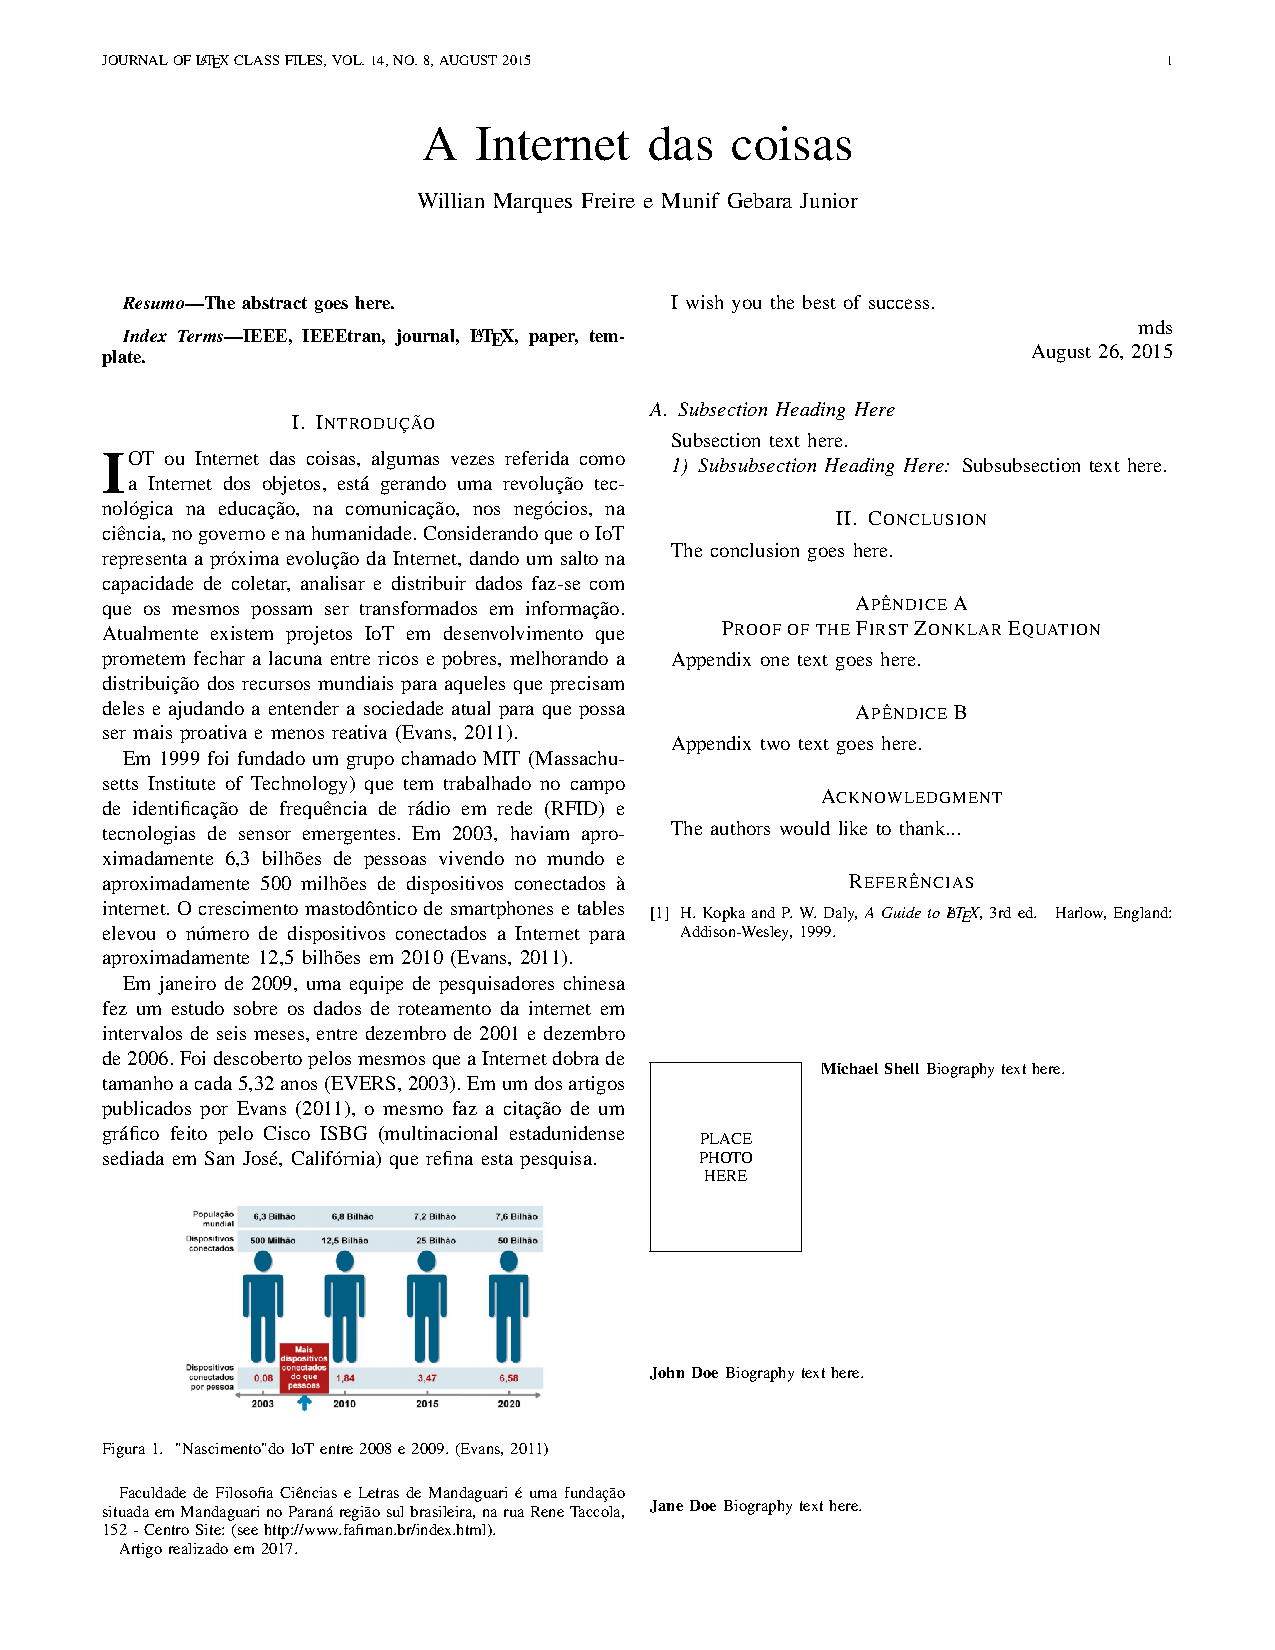
\includepdf[pages=-, offset=75 -75]{artigos/artigo1/bare_jrnl.pdf}
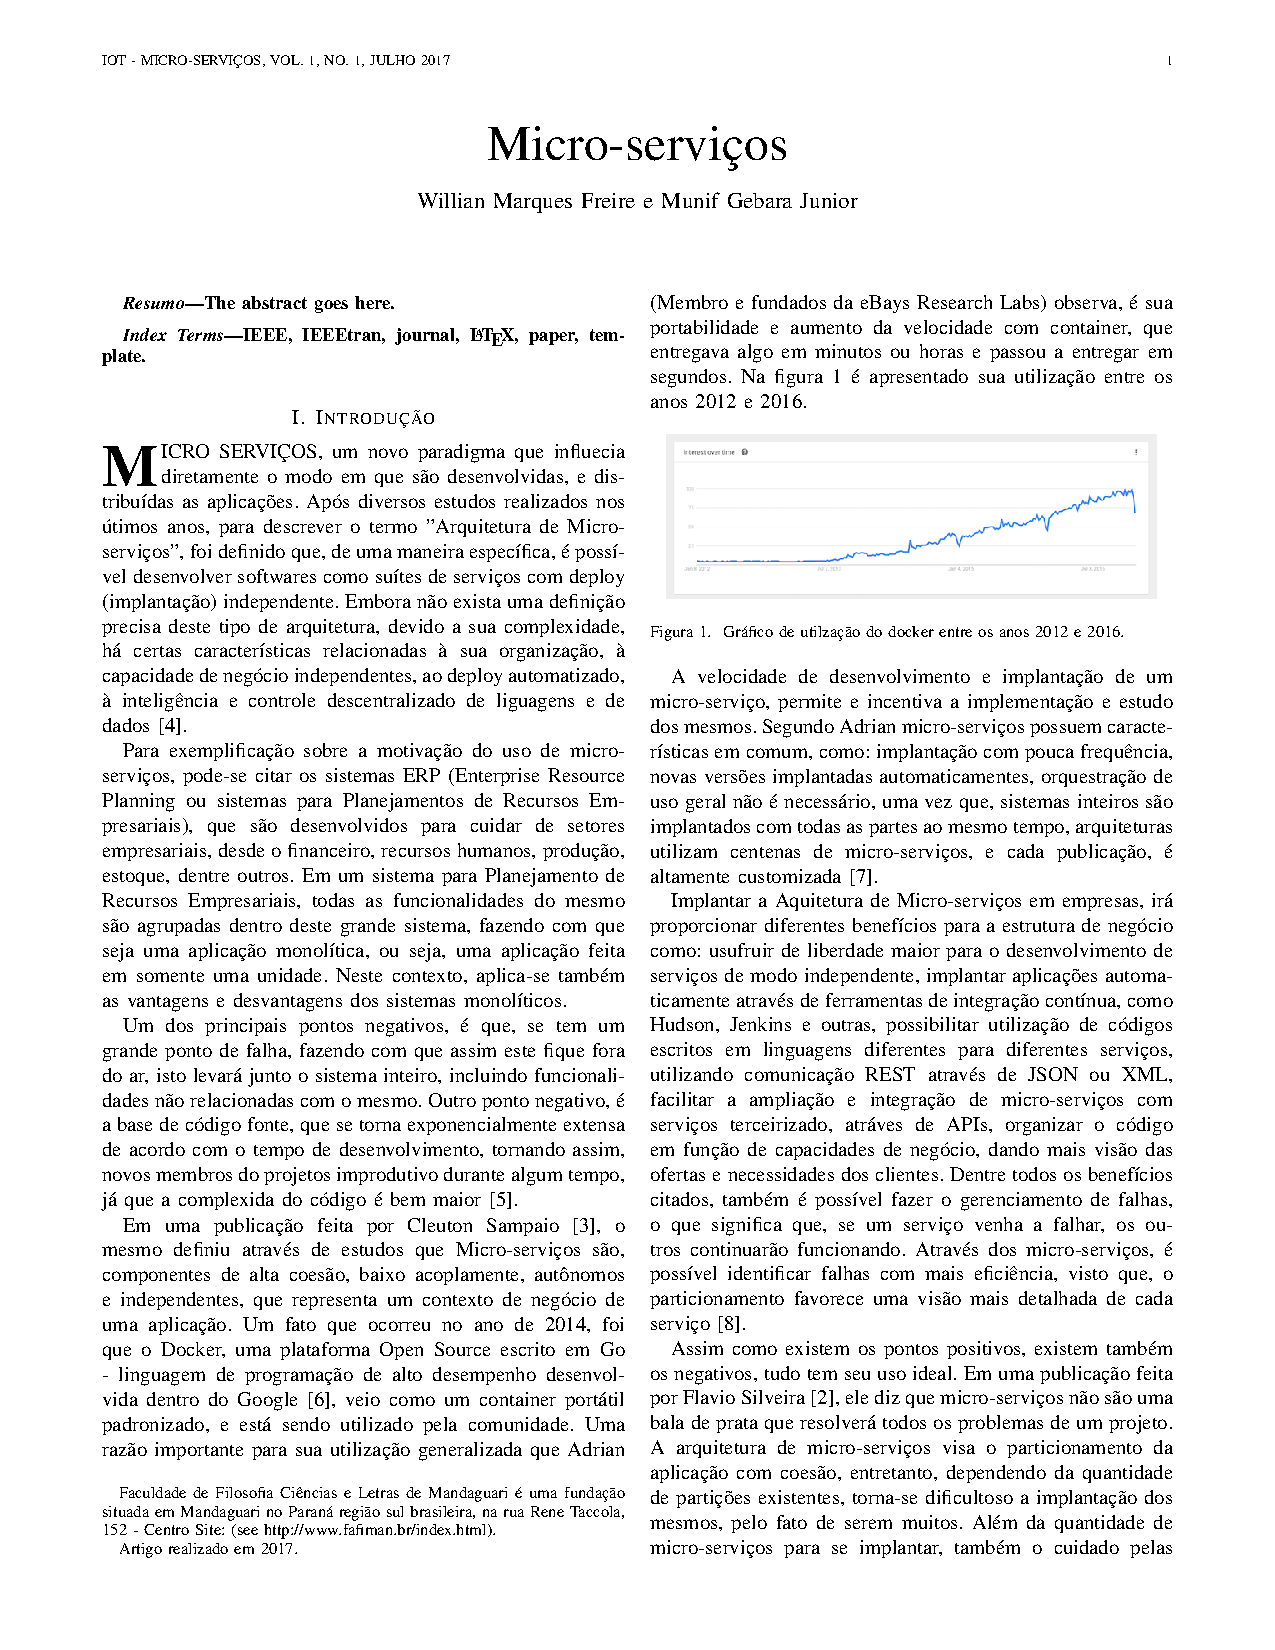
\includepdf[pages=-, offset=75 -75]{artigos/artigo2/bare_jrnl.pdf}
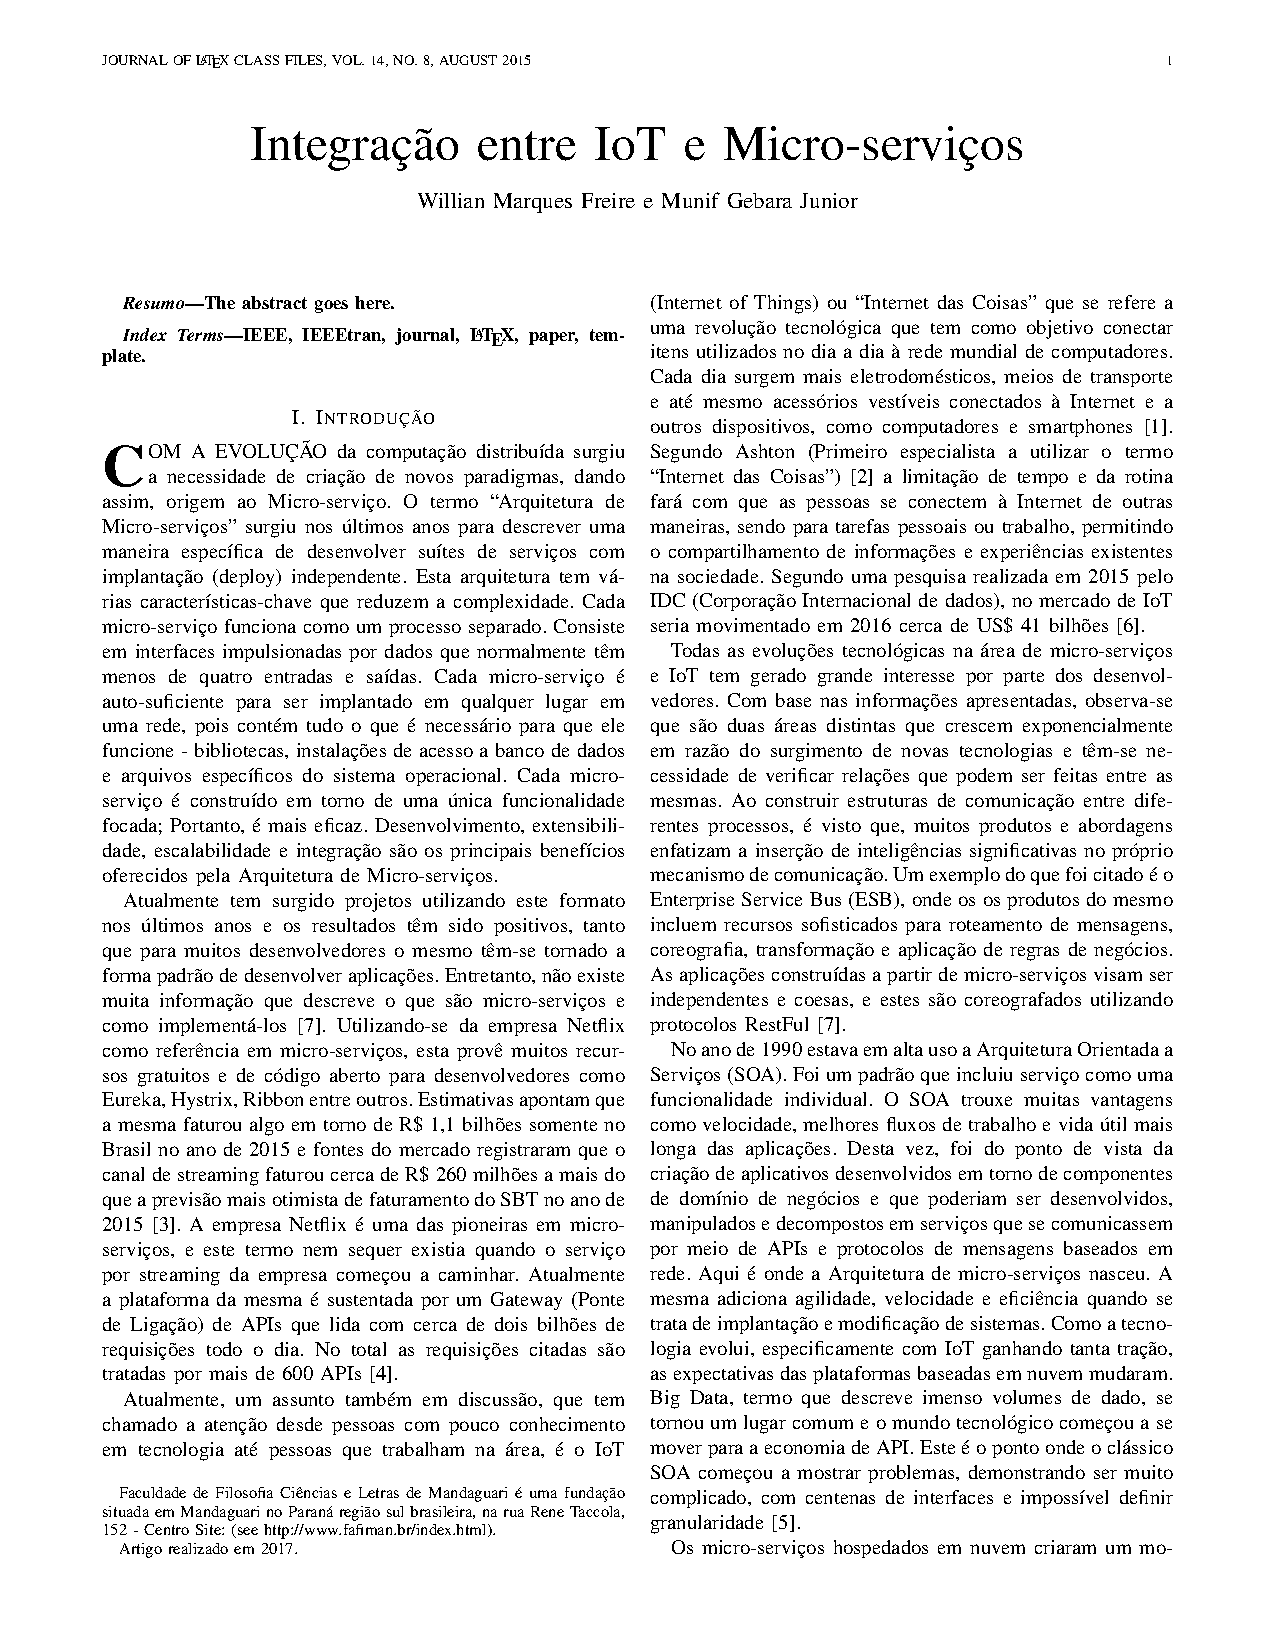
\includepdf[pages=-, offset=75 -75]{artigos/artigo3/bare_jrnl.pdf}

\setlength{\voffset}{0cm}
\setlength{\hoffset}{0cm}


\section{APRESENTAÇÃO E ANÁLISE DOS RESULTADOS}
Toda pesquisa deve apresentar uma análise sobre a investigação que foi realizada através da metodologia que foi aplicada. Nesta sessão é interessante inserir tabelas, gráficos, imagens que mostrem os resultados, análise de dados coletados, etc.

É interessante que nessa sessão o autor compare os seus resultados com os resultados de outros trabalhos existentes. Essa comparação aumenta a qualidade do trabalho e demonstra a relevância do mesmo. 

Nesta sessão o autor pode/deve incluir as contribuições científicas desenvolvidas tais como artigos, patentes, livros e outras contibuições que foram publicadas ou estão em fase de publicação e que são parte do trabalho.
\section{CONCLUSÕES E TRABALHOS FUTUROS}
A conclusão deve conter os principais aspectos e contribuições de forma a finalizar o trabalho apresentado. Deve-se apresentar o que era esperado do trabalho através dos objetivos inseridos inicialmente e mostrar o que foi conseguido. 

	Não deve-se inserir um novo assunto na conclusão. Aqui o autor apresentará as próprias impressões sobre o trabalho efetuado. 
    
É importante também que sejam identificadas limitações e problemas que surgiram durante o desenvolvimento do trabalho e quais as consequências do mesmo.

Os trabalhos futuros devem conter oportunidades de expansão do trabalho apresentado, bem como, novos projetos que puderam ser vislumbrados a partir do desenvolvimento do trabalho
%%%%%%%%%%%%%%%%%%%%%%%%%%%%% Referências %%%%%%%%%%%%%%%%%%%%%%%%%%%%%
\renewcommand{\refname}{\centering REFERÊNCIAS} %Centraliza nome Referencias%
\addcontentsline{toc}{section}{REFERÊNCIAS} %adiciona referencias ao sumario

\nocite{*}
\bibliographystyle{plainnat}

%%%%%%%%%%%%%%%%%%%%%%%%%%%%%%%%%%%%%%%%%%%%%%%%%%%%%%%%%%%%%%%%%%%%%%%

%%%%%%%%%%%%%%%%%%%%%%%%%%%%% ANEXO %%%%%%%%%%%%%%%%%%%%%%%%%%%%%
\section*{\centering{A – ANEXOS E APÊNDICES 1}}
\addcontentsline{toc}{section}{A - ANEXOS E APÊNDICES 1}

Anexos e apêndices são materiais adicionais, utilizados para complementar o texto, acrescentados ao final do trabalho, com a finalidade de esclarecimento ou de comprovação.

Apêndices são elaborados pelo autor e visam complementar uma argumentação. Os Anexos não são elaborados diretamente pelo autor e servem de fundamentação teórica, comprovação e ilustração (ex. mapas, leis, estatutos entre outros). Os apêndices devem aparecer antes dos anexos.

\bibliography{references}

\end{document}